%cSpell:disable
\subsection{Geodaten zu Hypotheken und Hochwasser}
\subsubsection{Hypothekengeodaten}

Für die Kompatibilität von Hypotheken- und Hochwasserdaten sind geografische Koordinaten erforderlich. Dieser Abschnitt befasst sich mit der Generierung präziser Koordinaten für die Datenpunkte.

Eine zufällige Verteilung in Bayern würde die Struktur eines Kreditportfolios nicht korrekt abbilden, da eine ungleichmäßige Verteilung von Immobilien sowohl in Deutschland als auch in Bayern zu beobachten ist. \textcite{zurek2022real} analysierte die Beziehung zwischen Bevölkerungsdichte und Kreditvergabe in Deutschland. Die Studie zeigt, dass Regionen mit stärkerem Wirtschaftswachstum höhere Immobilienpreise aufweisen. Dies führt zu einer erhöhten Kreditnachfrage. Auf Basis dieser empirischen Erkenntnisse wird die Bevölkerungsdichte als Grundlage für die Zuweisung spezifischer Koordinaten zu jedem Datenpunkt herangezogen.

Die verwendete Datenquelle stammt von \textcite{suche_postleitzahl}. Sie kombiniert OpenStreetMap-Daten mit Einwohnerzahlen von \textcite{destatis}. Dies ermöglicht eine präzise Segmentierung in Postleitzahlenzonen. Tabelle \ref{tab:geodaten} zeigt die Daten dieser geographischen Strukturierung.

\begin{table}[htbp]
    \centering
    \small  % Adjust font size to make everything fit in the table
    \caption{Übersicht der Geodaten für Postleitzahlgebiete in Bayern}
    \label{tab:geodaten}
    \begin{tabularx}{\textwidth}{lXcXcXc}
        \toprule
        \textbf{plz} & \textbf{einwohner} & \textbf{qkm} & \textbf{geometry} & \textbf{ort} & \textbf{landkreis} & \textbf{bundesland} \\
        \midrule
        81248 & 121  & 1984763  & POLYGON((…)) & München & & Bayern \\
        96103 & 8519 & 14585957   & POLYGON((…)) & Hallstadt & Landkreis Bamberg & Bayern \\
        63930 & 1552 & 16628516 & POLYGON((…)) & Neunkirchen & Landkreis Miltenberg & Bayern \\
        94530 & 2071 & 2414777 & POLYGON((…)) & Auerbach & Landkreis Deggendorf & Bayern \\
        85051 & 31592 & 3878506 & POLYGON((…)) & Ingolstadt & & Bayern \\
        63916 & 4002 & 51878059 & POLYGON((…)) & Amorbach & Landkreis Miltenberg & Bayern \\
        \dots & \dots & \dots & \dots & \dots & \dots & \dots \\
        83024 & 16249 & 9466746 & POLYGON((…)) & Rosenheim & & Bayern \\
        \bottomrule
    \end{tabularx}
\end{table}
\FloatBarrier

Tabelle \ref{tab:geodaten} wurde aus Shapefile-Daten der Postleitzahlenregionen generiert und umfasst die Bevölkerungsverteilung. Vier Spalten sind von besonderer Relevanz: Ort, Landkreis, Geometrie und Einwohner. Die Geometriespalte enthält die geografischen Koordinaten der Gemeinden, dargestellt als Polygon oder Multipolygon. Ein Multipolygon setzt sich aus mehreren Einzelpolygonen verschiedener Formen zusammen. Zur räumlichen Referenzierung dient das Koordinatensystem EPSG:3035. Abbildung \ref{fig:bevoelkerungsdichte} visualisiert die aus diesen Daten abgeleitete Bevölkerungsdichteverteilung Bayerns nach Postleitzahlenbereichen.

\begin{figure}[htbp]
    \centering
    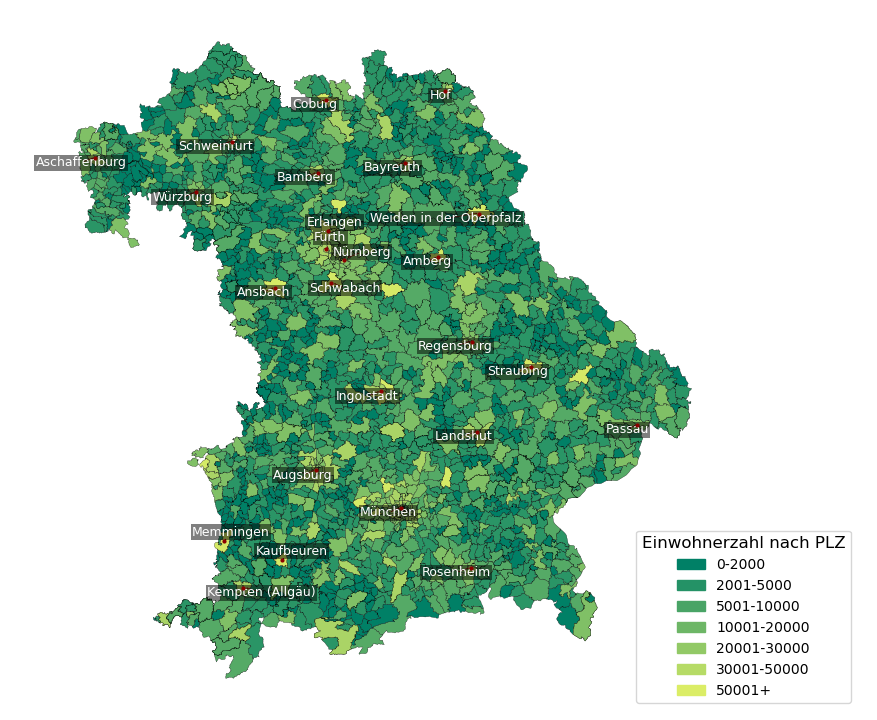
\includegraphics[width=0.95\textwidth]{figures/Bayern_pop_plz.png}
    \caption{Verteilung der Bevölkerungsdichte Bayerns nach Postleitzahlenbereichen}
    \label{fig:bevoelkerungsdichte}
\end{figure}
\FloatBarrier

Zur repräsentativen Verteilung der 3853 Datenpunkte, entsprechend der Anzahl der Hypothekarkredite, wird ein proportionaler Ansatz implementiert, der auf der Einwohnerzahl jeder Region basiert. Innerhalb der Postleitzahlgebiete erfolgt die Platzierung mittels eines kontrollierten stochastischen Verfahrens. Für jede Region wird eine zuvor determinierte Anzahl von Zufallspunkten innerhalb der definierten Gebietsgrenzen generiert. Jedem Punkt werden spezifische Koordinaten in Form von Latitude (Breitengrad) und Longitude (Längengrad) zugewiesen. Anschließend wird eine Verifikation der Lage innerhalb des jeweiligen Polygons durchgeführt. Bei erfolgreicher Validierung wird der Punkt mit seinen Latitude- und Longitude-Koordinaten in die Liste der akzeptierten Datenpunkte integriert. Die resultierenden Daten werden in Tabelle \ref{tab:geodatenhyp} dargestellt. Abbildung \ref{fig:hypothekenportfolio} zeigt die resultierende Distribution der Datenpunkte auf der Karte Bayerns.

\begin{table}[htbp]
    \centering
    \small  % Adjust font size to make everything fit in the table
    \caption{Übersicht der Geodaten für generierte Portfolios in Bayern}
    \label{tab:geodatenhyp}
    \begin{tabularx}{\textwidth}{lXlXrXr}
        \toprule
        \textbf{plz} & \textbf{ort} & \textbf{landkreis} & \textbf{latitude} & \textbf{longitude} \\
        \midrule
        637390 & Aschaffenburg & & 49.9725 & 9.1401 \\
        979040 & Dorfprozelten & Landkreis Miltenberg & 4.9711 & 9.3921 \\
        815470 & München & & 48.1047 & 11.5764 \\
        850980 & Großmehring & Landkreis Eichstätt & 48.7748 & 11.5158\\
        820640 & Oberhaching & Landkreis München & 47.9859 & 11.4903 \\
        863430 & Königsbrunn & Landkreis Augsburg & 48.2435 & 10.8994 \\
        972470 & Eisenheim & Landkreis Würzburg & 49.8850 & 10.1471 \\
        \dots & \dots & \dots & \dots & \dots \\
        852380 & Petershausen & Landkreis Dachau & 48.4000 & 11.5212\\
        \bottomrule
    \end{tabularx}
\end{table} 
\FloatBarrier

\begin{figure}[htbp]
    \centering
    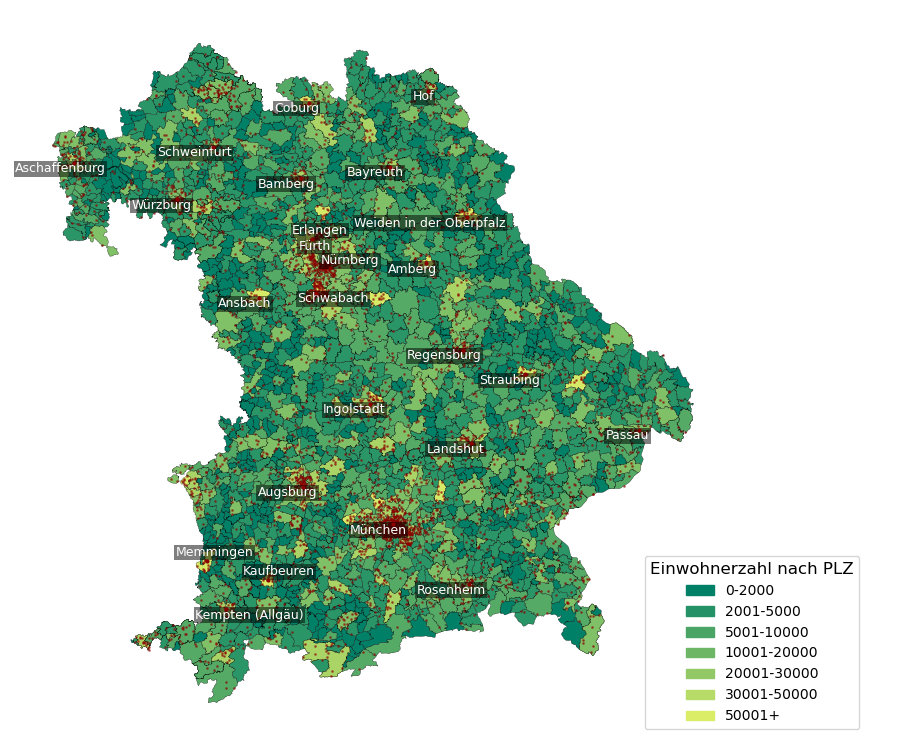
\includegraphics[width=\textwidth]{figures/bayern_por_pop.png} 
    \caption{Datenpunktverteilung im Hypothekenportfolio Bayern}
    \label{fig:hypothekenportfolio}
\end{figure}
\FloatBarrier

\subsubsection{Hochwassergeodaten}\label{sec:hochgeo}
Nach der Erfassung der geographischen Koordinaten der Hypothekendarlehen ist es erforderlich, die Lage der entsprechenden Immobilien in Bezug auf Hochwasserrisikogebiete zu ermitteln. Infolgedessen erläutert dieser Abschnitt die Methodologie zur Erstellung einer detaillierten Hochwasserrisikokarte für Bayern. Diese basiert auf EU-Stresstest-Szenarien sowie regionalen Daten und beschreibt die Integration diverser Datenquellen zur präzisen Risikoanalyse.

Im Rahmen eines EU-weiten Stresstests stellt die \ac{EZB} den Banken zur Simulation eines schweren Überschwemmungsszenarios eine Hochwasserrisikokarte (Abbildung \ref{fig:euflut}) zur Verfügung.

\begin{figure}[htbp]
    \centering
    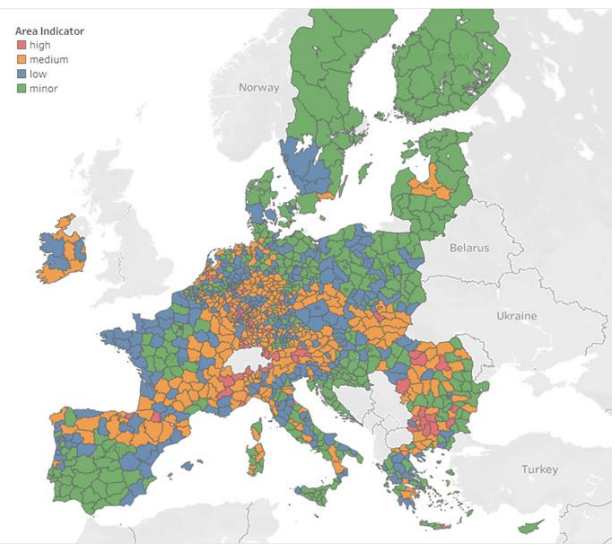
\includegraphics[width=\textwidth]{figures/euflood.png} 
    \caption{EU-Hochwasserrisikokarte.Quelle: EZB 2022 Klimarisiko-Stresstest}
    \label{fig:euflut}
\end{figure}
\FloatBarrier

Diese Karte basierend auf Informationen der Gemeinsamen Forschungsstelle der Europäischen Kommission und ergänzt durch Daten von Four Twenty Seven kategorisiert Regionen nach Risikoklassen \parencite{ECB2022ClimateStressTest}. Da jedoch die zugrundeliegenden Daten von der \ac{EZB} nicht veröffentlicht wurden und die visuelle Repräsentation keine präzise Identifikation spezifischer Regionen ermöglicht, erweist sich für Bayern die Notwendigkeit einer differenzierteren Analyse als evident. 

Als potenzielle Lösung für diese Problematik könnten die vom Bayerischen Landesamt für Umwelt im Rahmen des Hochwasserrisikomanagements entwickelten Kartierungen herangezogen werden. Diese spezifischen Kartierungen für die Einzugsgebiete von Donau, Rhein und Elbe bieten eine detaillierte Darstellung der Hochwassergefährdung, der potenziell betroffenen Landnutzungen sowie historischer Hochwasserereignisse, wodurch eine präzisere regionale Risikoeinschätzung ermöglicht wird \parencite{LfU_Bayern}.
Die ursprünglich im ETRS89-Koordinatensystem vorliegenden Daten werden für die Analyse in das EPSG:3035-System konvertiert. Diese Transformation ermöglicht eine präzise Integration und Darstellung aller Datensätze auf einer einheitlichen Karte Bayerns.
Eine abschließende Abbildung \ref{fig:bayernflut} präsentiert einen umfassenden Überblick über die potenziell von Hochwasser betroffenen Gebiete in Bayern, wodurch die räumliche Verteilung des Risikos verdeutlicht wird.
\begin{figure}[htbp]
    \centering
    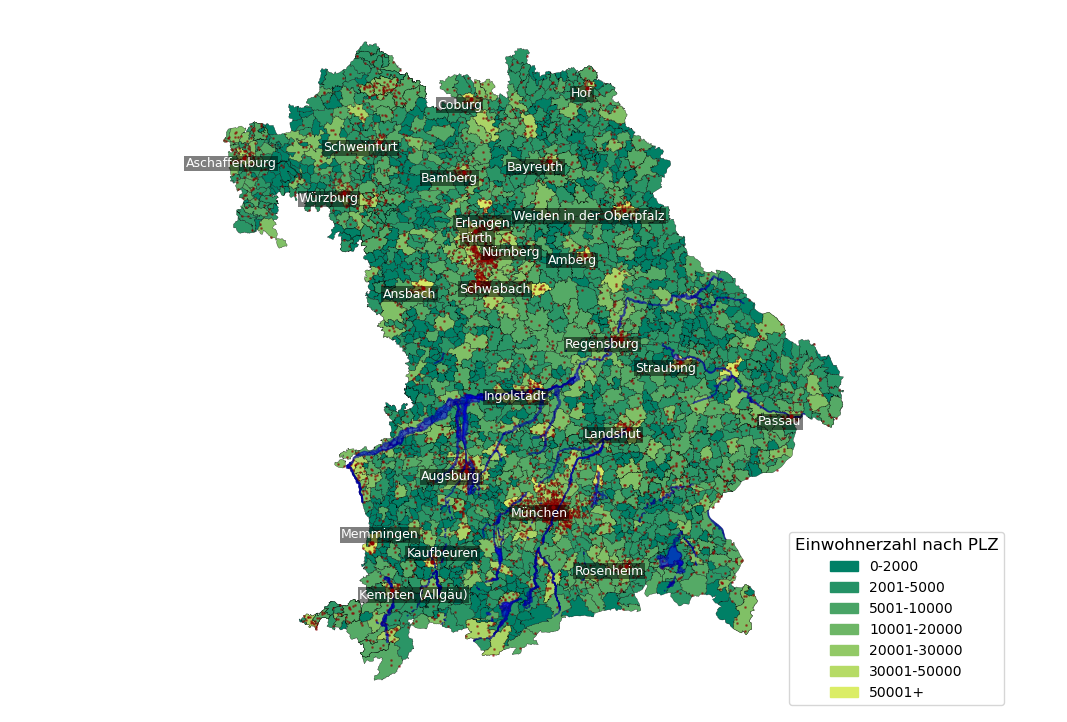
\includegraphics[width=\textwidth]{figures/bayern_flut.png} 
    \caption{Visualisierung historischer Hochwasserereignisgebiete und Verteilung des Darlehensportfolios in Bayern}
    \label{fig:bayernflut}
\end{figure}
\FloatBarrier


